\chapter{Motivation} \label{chapter:MOTIVATION}

In the Lively Kernel, programmers can create applications by manipulating and composing graphical parts.
The development of such parts and related recovery needs are shown by example in this chapter.

\section{Part Development By Example}

To exemplify how developers change objects directly in Lively, we will outline the process of adding a new feature to Lively's Object Editor.

\begin{figure}[h]
    \centering
    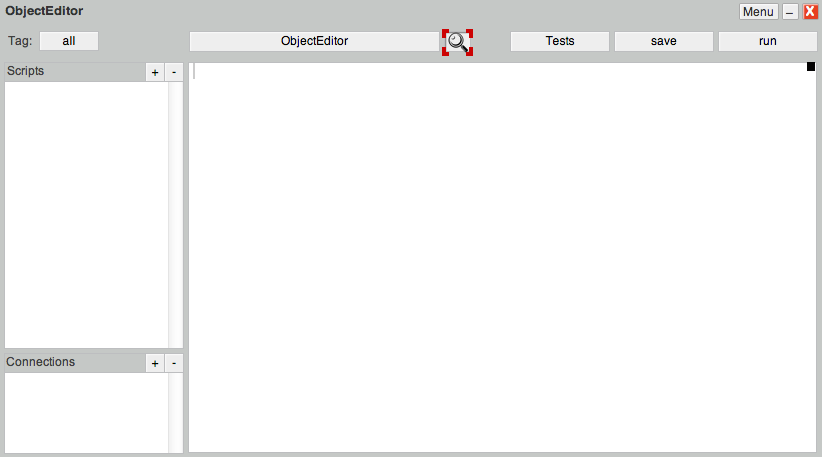
\includegraphics[width=\textwidth]{figures/3_motivation/1_magnifierButton.png}
    \caption{The Object Editor with its magnifier button highlighted with a red outline.}
    \label{fig:MagnifierButton}
\end{figure}

The new feature we add in this example is a magnifier button that can show the editor's current target.
The target is the object to which the Object Editor currently presents scripts to and allows to manipulate.
This requires to create and add a new button morph to the editor, shown in Figure~\ref{fig:MagnifierButton}.

\begin{figure}[h]
    \centering
    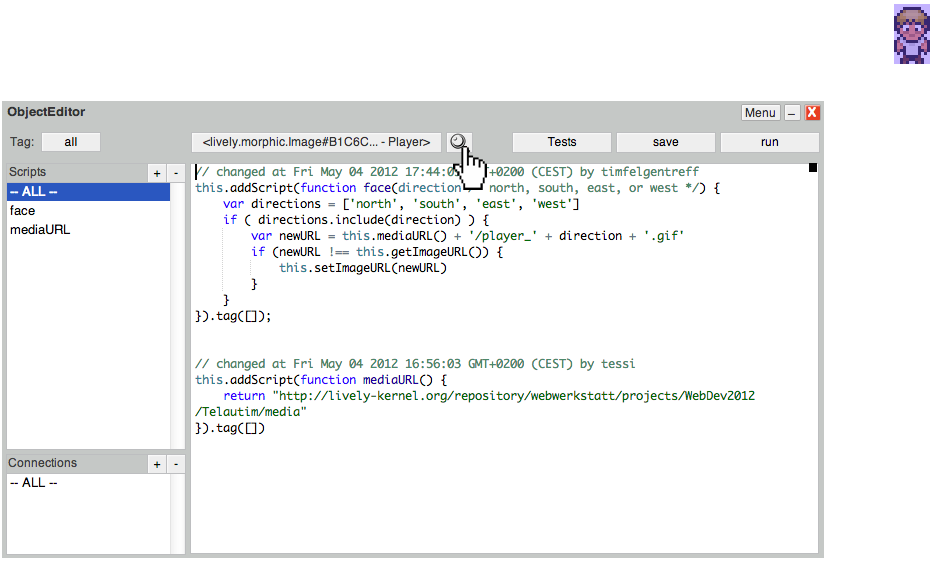
\includegraphics[width=\textwidth]{figures/3_motivation/2_magnifierBehavior.png}
    \caption{Hovering a button of the Object Editor highlights the editor's current target.}
    \label{fig:MagnifierBehavior}
\end{figure}

The magnifier button implements two features: First, when a programmer hovers over the button, the Object Editor's current target object is highlighted through a blue and transparent overlay. Second, when a programmer clicks the button, the current target selection is revoked and the programmer can visually select the new target of the editor.
This example covers the first of these two behaviors, which is shown in Figure~\ref{fig:MagnifierBehavior}.

The editor itself has been been developed by composing and editing graphical objects directly.
For this reason, we do not have to adapt any source code modules to change the editor, but rather manipulate and save the concrete object the editor is.

\paragraph{Manipulating the Button Morph}
First, we manipulate the visual appearance of a button, as shown in Figure~\ref{fig:ButtonBuilding}.
The button in \textcircled{1} can be found in the Lively Kernel's Parts Bin repository.
We then can use the button's halos and, in particular, the resize tool in \textcircled{2} to give the button a smaller and square extent.
Next, we can load an image showing a magnifier.
Using drag and drop we can add the image to the button and the button to the editor, as done in \textcircled{3}.
Dropping a morph onto another structurely connects morphs in Lively.
That is, moving the editor around will also move the button with its image accordingly, while saving will respectively include both the button and the image.
Subsequentely, we can add the result of these direct manipulations, visible in \textcircled{4}, to the object editor.

\begin{figure}[h]
    \centering
    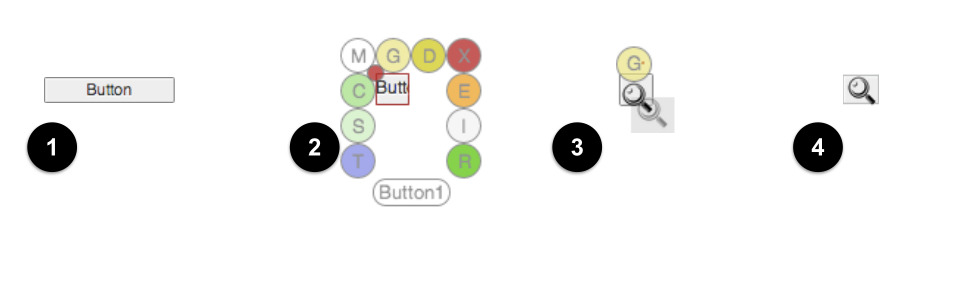
\includegraphics[width=\textwidth]{figures/3_motivation/3_buildingTheButton.png}
    \caption{Directly manipulating a button morph.}
    \label{fig:ButtonBuilding}
\end{figure}

All these changes are made directly to the state of objects: the button morph, the magnifier image morph, and the editor morph.
When programmers edit parts directly in this way, they often see the effects of their actions immediately.
For example, when adding the button morph to the Object Editor, where the button will be added is visible at all times.
Developers do not need to run any code to check the resulting appearance.

\paragraph{Scripting the Button Morph}
Next, the magnifier button needs its behavior.
We add scripts to the button to lay a translucent rectangle over the current target, highlighting the morph that is currently being edited.
This behavior can be triggered from two other scripts of the button morph, \lstinline{onMouseMove} and \lstinline{onMouseOut}.
These two scripts make sure that the overlay is shown only on hover.

Such scripts can be added using another Object Editor.
The editor also allows to evaluate code in the context of its target.
So, when developers want to test a script or even just specific lines of code, they can often try the behavior directly with the actual target.


\section{Recovery Needs When Developing Parts}

\todo{this whole section needs to be more concrete and actually present situations from the previously introduced example. e.g. explain how parts of the script to can be evaluated to test whether the overlay works, but even when that works as intented there is then just wrong state (an overlay added to some morph in the world..)}

While manipulating objects directly, developers might make changes to object state that they subsequentely want to undo.
In the previously summarized example developers might, for example, accidentally move the new button after carefully positioning it.
Or they might accidentally drop the button into an existing layout, thereby undesirably repositioning multiple unrelated morphs.
An extreme example for such an accidental inappropriate change is closing a morph that had meaningful, but unsaved changes.

In constrast to those clearly undesired, accidental changes, well-intentioned changes can also result in the desire to recover a previous development state.
For example, when fine-tuning the visual appearance of a morph, a developer might make many changes to the sizes, the positions, and the colors of morphs, only to decide later-on that a particular intermediate version was most appealing.
Or developers edit a script only to learn that the change introduced an an error or a decrease in performance.
Further, developers can change objects not only through direct manipulation, but also could write a code snippet that makes changes to the state or behavior of an objects.
Such a snippet could of course change any number of properties of many objects at once, so re-establishing a previous situation would be a laborious task.

Another category of development interactions that potentially introduce undesirable changes is the exploration of code snippets.
As Lively's Object Editor manipulates the scripts of a specific object, developers can often evaluate the scripts or parts of them directly.
While such code evaluation might help to understand the effects of particular code, it might also actually change the editor's target or other objects undesirably and permanently.

In essence, there are many situations in which developers might want to undo some of their operations.
They might want to recover a previous development state or just withdraw particular changes to particular objects.
Developers can save particular versions of objects and those can be restored later-on by, for example, using Lively's Parts Bin.
However, explicitly saving particular versions of objects has several drawbacks.


\todo{this section's end should provide a concrete idea of the recovery needs: developers want to be able to just go back to previous state. show this with before and after screenshots of the visual applications, but then also provide a before-and-after on the level of objects (conceptual graphic)}


% When programmers unexpectedly introduce problems to the functionality, performance, or design of their applications, they might want to recover a previous development state.
% In programming systems like the Lively Kernel, where programmers often work at runtime on objects, a development state consists of the state of objects, which includes object-specific behavior.
% To be able to recover such a development state, comprehensive recovery support for the Lively Kernel must, therefore, preserve versions of objects.
